\documentclass[serif, aspectratio=169]{beamer}
\usepackage[T1]{fontenc}
\usepackage{fourier}
\usepackage{hyperref}
\usepackage{latexsym,amsmath,xcolor,multicol,booktabs,calligra}
\usepackage{graphicx,listings,stackengine}
\usepackage{lipsum}
\usepackage[english]{babel}
\usepackage[utf8]{inputenc}
\usepackage{array}
\usepackage{ragged2e}
\usepackage{subfigure}
\usepackage{longtable}
\usepackage{etoolbox}
\usepackage{lscape}
\usepackage{algorithm}
\usepackage{algpseudocode}
\usepackage{multirow}
\usepackage{adjustbox}
\usepackage{tabularx}
\usepackage{amssymb,amsfonts}
\usepackage{textcomp}
\usepackage{mathtools}
\usepackage{bibentry}

\author{Scholar Name: Devansh Vishwa \texorpdfstring{\\}{, }Registration No.: 2502010003 }
\title{Cross-Dataset Generalization and Explainability of Lightweight CNNs for 12-Lead ECG Classification}

\institute{
	Supervisor: Dr. Amit Kumar Bairwa, Department of AIML \\
	\begin{figure}[htpb]
		\begin{center}
			\includegraphics[keepaspectratio, scale=0.2]{pic/MUJ.png}
		\end{center}
	\end{figure}
	\textbf{Faculty of Science, Technology and Architecture} \\
	\textbf{School of CSE, Department of CSE}\\
	\textbf{Manipal University Jaipur, Rajasthan, India} \\ \vspace{5mm}
	\textbf{November 2026}
}
\usepackage{HKUSTstyle}

\def\cmd#1{\texttt{\color{red}\footnotesize $\backslash$#1}}
\def\env#1{\texttt{\color{blue}\footnotesize #1}}
\definecolor{hkustyellow}{RGB}{167, 131, 55}
\definecolor{hkustblue}{RGB}{0, 56, 116}
\definecolor{hkustred}{RGB}{209, 51, 59}

\begin{document}
\justify

% --- Title Slide ---
\begin{frame}
	\titlepage
\end{frame}

% --- Table of Contents ---
\begin{frame}
	\tableofcontents[sectionstyle=show,
	subsectionstyle=show/shaded/hide,
	subsubsectionstyle=show/shaded/hide]
\end{frame}

% =====================================================
\section{Introduction}
% =====================================================

\begin{frame}{Introduction}
	\frametitle<presentation>{Introduction: The 12-Lead ECG and Automated Interpretation}
	\begin{itemize}
		\item \textbf{What is an ECG?}
		\begin{itemize}
			\item The electrocardiogram (ECG) records the electrical activity of the heart. A standard 12-lead ECG views the heart from 12 directions over 10 seconds.
			\item Each heartbeat appears as a P-wave (atrial activation), a QRS complex (ventricular activation) and a T-wave (ventricular recovery).
		\end{itemize}
		\item \textbf{Why automate ECG interpretation?}
		\begin{itemize}
			\item Cardiovascular disease is the leading cause of death worldwide, and the ECG is the most common first-line cardiac test.
			\item Expert interpretation is slow and not available everywhere; deep learning models can screen ECGs in milliseconds.
		\end{itemize}
		\item \textbf{The catch:} a model that performs well on data from one hospital often performs worse on data from another hospital.
	\end{itemize}
\end{frame}

% =====================================================
\section{Problem Statement}
% =====================================================

\begin{frame}{Problem Statement}
	\frametitle<presentation>{Problem Statement}
	\begin{itemize}
		\item \textbf{Domain shift between hospitals}
		\begin{itemize}
			\item ECG devices, filters, electrode placement and patient populations differ between hospitals.
			\item PTB-XL (Germany, Schiller devices) and Chapman-Shaoxing/Ningbo (China, GE MUSE) are a realistic example of this shift.
		\end{itemize}
		\item \textbf{Label and prevalence shift}
		\begin{itemize}
			\item The two datasets use different label vocabularies (SCP-ECG vs SNOMED-CT).
			\item Class prevalence changes strongly, e.g. atrial flutter is 0.3\% of PTB-XL but 17.9\% of Chapman.
		\end{itemize}
		\item \textbf{Black-box decisions}
		\begin{itemize}
			\item Clinicians need to know whether a model looks at physiologically meaningful parts of the ECG (P, QRS, T) or at noise.
		\end{itemize}
	\end{itemize}
\end{frame}

% =====================================================
\section{Objective}
% =====================================================

\begin{frame}{Objective}
	\frametitle<presentation>{Objectives}
	\textbf{How do we intend to study this problem?}\par
	\begin{itemize}
		\item \textbf{Fair benchmark:} Train four parameter-matched 1D CNNs (about 0.5M parameters each) under one identical data, preprocessing, training and evaluation protocol.
		\item \textbf{Zero-shot external test:} Train only on PTB-XL and test on Chapman-Shaoxing/Ningbo without any fine-tuning or threshold re-tuning.
		\item \textbf{Proposed model:} Design PhysioDKS-IncepSE, a physiologically initialised multi-scale front-end on top of an Inception + Squeeze-and-Excitation backbone.
		\item \textbf{Explainability:} Measure, with numbers, where the models look (QRS, P/T, baseline) and which leads they rely on.
	\end{itemize}
\end{frame}

\begin{frame}{Hypotheses}
	\frametitle<presentation>{Hypotheses Tested}
	\begin{itemize}
		\item \textbf{H1:} A standard CNN (ResNet1D) loses the most performance under hospital shift.
		\item \textbf{H2:} The physiological Stage-1 front-end (dynamic kernel selection + InstanceNorm) reduces the cross-dataset performance gap.
		\item \textbf{H3:} The proposed model improves both in-domain and cross-dataset performance.
		\item \textbf{H4:} The proposed model focuses on P/QRS/T waves rather than noise.
	\end{itemize}
\end{frame}

% =====================================================
\section{Literature Review}
% =====================================================

\begin{frame}{Literature Review: Existing Studies}
	\frametitle<presentation>{Literature Review}
	\begin{table}[h]
		\centering
		\caption{Literature Review}
		\renewcommand{\arraystretch}{1.25}
		\resizebox{\textwidth}{!}{
		\begin{tabular}{|l|l|l|l|}
			\hline
			\textbf{Author(s)} & \textbf{Data / Application} & \textbf{Method} & \textbf{Work / Contribution} \\
			\hline
			Wagner et al. \cite{wagner2020ptbxl} & PTB-XL, 21,837 ECGs & Dataset & Public 12-lead dataset with patient-wise folds \\
			\hline
			Strodthoff et al. \cite{strodthoff2021} & PTB-XL & ResNet, Inception, LSTM & Standard benchmark and evaluation protocol \\
			\hline
			Zheng et al. \cite{zheng2020chapman} & Chapman-Shaoxing & Dataset & 12-lead arrhythmia database, 10,000+ patients \\
			\hline
			Reyna et al. \cite{reyna2022issues} & Multi-source ECGs & Challenge analysis & Label and population heterogeneity across datasets \\
			\hline
			Ismail Fawaz et al. \cite{fawaz2020inceptiontime} & Time series & InceptionTime & Multi-scale convolution kernels \\
			\hline
			Hu et al. \cite{hu2018se} & Images & SE attention & Channel re-weighting (Squeeze-and-Excitation) \\
			\hline
			Selvaraju et al. \cite{selvaraju2017gradcam} & Images & Grad-CAM & Gradient-based visual explanations \\
			\hline
		\end{tabular}
		}
	\end{table}
\end{frame}

\begin{frame}{Research Gap}
	\frametitle<presentation>{Research Gap}
	\begin{itemize}
		\item Most PTB-XL studies report only in-domain results on fold 10; external validation on a different hospital is rare.
		\item Model comparisons are often confounded by different preprocessing, training settings and parameter counts.
		\item Accuracy drops on external data are rarely decomposed into ranking loss (AUC) and threshold/calibration loss (F1).
		\item Explainability is usually shown as a few selected heatmaps, without quantitative, class-wise evaluation.
	\end{itemize}
\end{frame}

% =====================================================
\section{Methodology}
% =====================================================

\begin{frame}{Datasets}
	\frametitle<presentation>{Datasets and Label Harmonization}
	\begin{itemize}
		\item \textbf{Source (training):} PTB-XL v1.0.1. Folds 1--8 train (17,441 ECGs), fold 9 validation (2,193), fold 10 test (2,203). No patient appears in more than one split.
		\item \textbf{Target (zero-shot test):} PhysioNet \texttt{ecg-arrhythmia} v1.0.0 (Chapman-Shaoxing + Ningbo), 45,151 ECGs. Never used for training or tuning.
		\item \textbf{Label set (rhythm9):} NSR, AFIB, AFL, RBBB, LBBB, PAC, PVC, STach, SBrady. PTB-XL SCP-ECG codes and Chapman SNOMED-CT codes were mapped to one common label set.
	\end{itemize}
	\begin{table}[h]
		\centering
		\renewcommand{\arraystretch}{1.1}
		\resizebox{\textwidth}{!}{
		\begin{tabular}{|l|c|c|c|c|c|c|c|c|c|}
			\hline
			 & NSR & AFIB & AFL & RBBB & LBBB & PAC & PVC & STach & SBrady \\
			\hline
			PTB-XL train positives & 13,426 & 1,211 & 59 & 433 & 428 & 318 & 916 & 661 & 509 \\
			\hline
			Prevalence PTB-XL (\%) & 76.9 & 6.9 & 0.3 & 2.5 & 2.5 & 1.8 & 5.3 & 3.8 & 2.9 \\
			\hline
			Prevalence Chapman (\%) & 18.0 & 3.9 & 17.9 & 3.9 & 1.0 & 2.9 & 3.1 & 16.1 & 36.7 \\
			\hline
		\end{tabular}
		}
	\end{table}
\end{frame}

\begin{frame}{Label Shift}
	\frametitle<presentation>{Label Prevalence Shift Between Datasets}
	\begin{figure}[htbp]
		\centering
		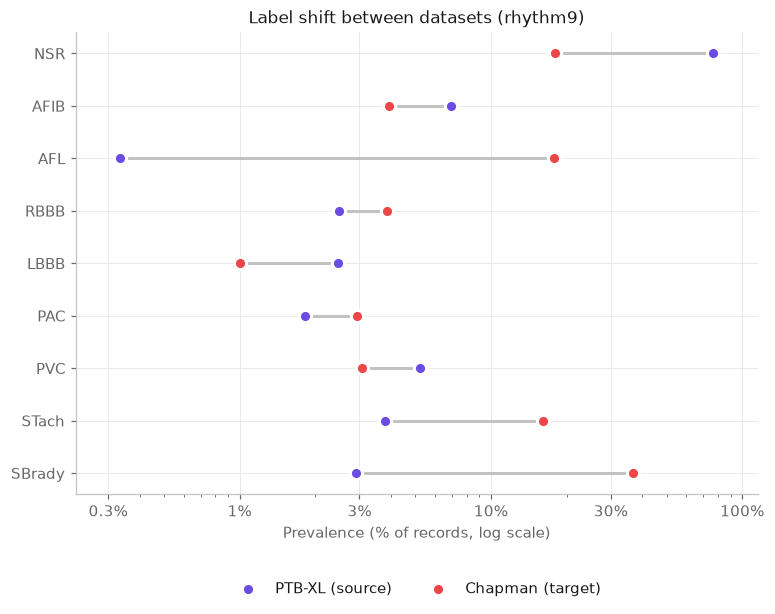
\includegraphics[width=0.5\linewidth]{figs/label_shift.png}
		\caption{Class prevalence in PTB-XL (source) and Chapman (target), log scale.}
	\end{figure}
\end{frame}

\begin{frame}{Preprocessing}
	\frametitle<presentation>{Preprocessing (Identical for Both Datasets)}
	\begin{columns}[c]
		\begin{column}{0.5\textwidth}
			\begin{itemize}
				\item \textbf{Units and leads:} signals converted to mV; leads reordered by name to I, II, III, aVR, aVL, aVF, V1--V6.
				\item \textbf{Sampling:} 100 Hz, 10 s (1000 samples). Chapman resampled from 500 Hz to 100 Hz.
				\item \textbf{Filtering:} zero-phase Butterworth band-pass, 0.5--40 Hz, order 4.
				\item \textbf{Normalization:} per-record, per-lead z-score.
			\end{itemize}
		\end{column}
		\begin{column}{0.48\textwidth}
			\begin{figure}[htbp]
				\centering
				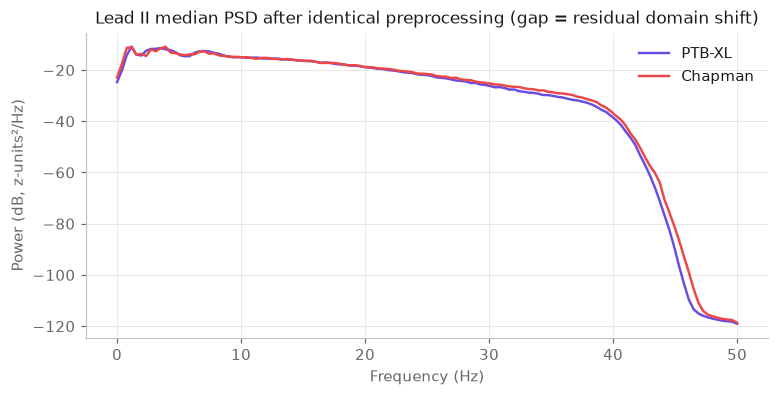
\includegraphics[width=\linewidth]{figs/psd_after_preprocessing.png}
				\caption{Lead II median power spectrum after preprocessing.}
			\end{figure}
		\end{column}
	\end{columns}
\end{frame}

\begin{frame}{Models}
	\frametitle<presentation>{Models Compared}
	All four models use the same input (12 $\times$ 1000) and the same head (global average pooling, dropout, linear layer). Only the body differs.
	\begin{table}[h]
		\centering
		\renewcommand{\arraystretch}{1.2}
		\resizebox{0.9\textwidth}{!}{
		\begin{tabular}{|l|l|c|l|}
			\hline
			\textbf{Model} & \textbf{Role} & \textbf{Params} & \textbf{Key idea} \\
			\hline
			ResNet1D \cite{he2016resnet} & Baseline & 0.55M & Standard residual CNN with strided downsampling \\
			\hline
			InceptionTime \cite{fawaz2020inceptiontime} & Base architecture & 0.47M & Multi-scale kernels (39/19/9) with residual connections \\
			\hline
			IncepSE & Ablation & 0.48M & InceptionTime + Squeeze-and-Excitation \cite{hu2018se} \\
			\hline
			PhysioDKS-IncepSE & Proposed & 0.49M & Physiological Stage-1 front-end + IncepSE backbone \\
			\hline
		\end{tabular}
		}
	\end{table}
	\begin{itemize}
		\item InceptionTime $\rightarrow$ IncepSE measures the effect of SE attention.
		\item IncepSE $\rightarrow$ PhysioDKS-IncepSE measures the effect of the Stage-1 front-end.
	\end{itemize}
\end{frame}

\begin{frame}{Proposed Model}
	\frametitle<presentation>{Proposed Model: PhysioDKS-IncepSE}
	\begin{itemize}
		\item \textbf{Stage 1: Physiological multi-scale DKS filter (per lead)}
		\begin{itemize}
			\item Three kernel sizes matched to ECG wave durations at 100 Hz: k = 5 (50 ms, R-peak/QRS upstroke), k = 11 (110 ms, full QRS), k = 21 (210 ms, P- and T-waves).
			\item Four filters per lead per branch, initialised as Gaussian-derivative wavelets and fine-tuned during training.
			\item Dynamic Kernel Selection (DKS): learned attention weights decide how much each kernel size contributes for each record.
			\item InstanceNorm to remove per-record amplitude and offset differences; Lead-SE gate to weight the 12 leads.
		\end{itemize}
		\item \textbf{Stage 2: IncepSE backbone}
		\begin{itemize}
			\item Six Inception modules (kernels 39/19/9) with Squeeze-and-Excitation channel attention and residual connections.
		\end{itemize}
		\item \textbf{Head:} global average pooling, dropout (0.3), linear layer with 9 sigmoid outputs (multi-label).
	\end{itemize}
\end{frame}

% =====================================================
\section{Experimental Setup}
% =====================================================

\begin{frame}{Experimental Setup (1/2)}
	\frametitle{Training Protocol (Same for All Models)}
	\begin{columns}[c]
		\begin{column}{0.45\textwidth}
			\begin{itemize}
				\item \textbf{Loss:} binary cross-entropy (multi-label).
				\item \textbf{Optimizer:} AdamW, weight decay $10^{-2}$.
				\item \textbf{Schedule:} OneCycleLR, max learning rate $10^{-3}$.
				\item \textbf{Other:} mixed precision, gradient clipping 1.0, early stopping (patience 8), seed 42.
				\item \textbf{Model selection:} best validation (fold 9) macro-AUC.
				\item \textbf{Hardware:} NVIDIA RTX 3050 6 GB; total training about 31 min; inference 0.25--0.48 ms per ECG.
			\end{itemize}
		\end{column}
		\begin{column}{0.53\textwidth}
			\begin{figure}[htbp]
				\centering
				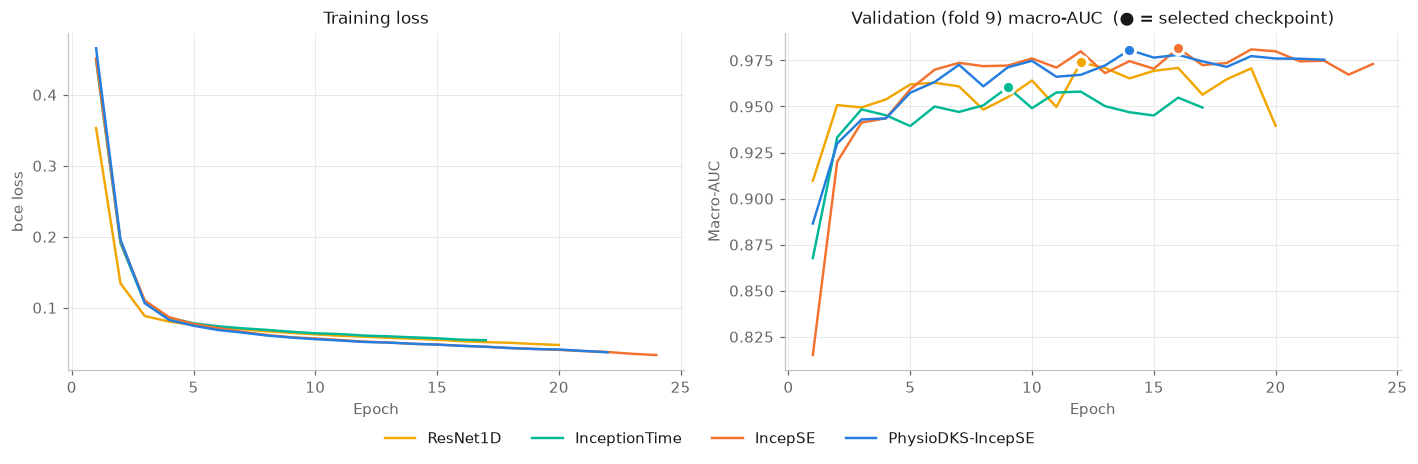
\includegraphics[width=\linewidth]{figs/training_curves.png}
				\caption{Training loss and validation macro-AUC.}
			\end{figure}
		\end{column}
	\end{columns}
\end{frame}

\begin{frame}{Experimental Setup (2/2)}
	\frametitle{Evaluation Metrics}
	\textbf{Primary Metric:}
	\begin{itemize}
		\item Macro-AUC (threshold-free, average of per-class ROC-AUC)
	\end{itemize}
	\textbf{Secondary Metrics:}
	\begin{itemize}
		\item Macro-F1, Sensitivity, Specificity, AUPRC
		\item Generalization gap: $\Delta$AUC = AUC(PTB-XL fold 10) $-$ AUC(Chapman)
	\end{itemize}
	\textbf{Protocol:}
	\begin{itemize}
		\item Per-class thresholds tuned only on PTB-XL fold 9 and applied unchanged to fold 10 and Chapman.
		\item 95\% confidence intervals and p-values from 1000 paired bootstrap resamples.
		\item Oracle F1 (thresholds tuned on Chapman itself) is reported for analysis only; it is not deployable.
	\end{itemize}
\end{frame}

% =====================================================
\section{Results}
% =====================================================

\begin{frame}{Results: Threshold-Free Metrics}
	\frametitle<presentation>{Main Results: Macro-AUC}
	\begin{table}[h]
		\centering
		\caption{In-domain (PTB-XL fold 10) and zero-shot (Chapman) performance, 95\% CI in brackets}
		\renewcommand{\arraystretch}{1.2}
		\resizebox{\textwidth}{!}{
		\begin{tabular}{|l|c|c|c|c|c|c|}
			\hline
			\textbf{Model} & \textbf{Params} & \textbf{PTB-XL Macro-AUC} & \textbf{Chapman Macro-AUC} & \textbf{$\Delta$AUC (gap)} & \textbf{PTB-XL AUPRC} & \textbf{Chapman AUPRC} \\
			\hline
			ResNet1D & 0.55M & 0.961 [0.948, 0.972] & 0.880 [0.877, 0.883] & 0.082 [0.069, 0.092] & 0.753 & 0.548 \\
			\hline
			InceptionTime & 0.47M & 0.946 [0.930, 0.959] & 0.908 [0.905, 0.910] & 0.038 [0.023, 0.052] & 0.733 & 0.572 \\
			\hline
			IncepSE & 0.48M & 0.968 [0.955, 0.979] & 0.929 [0.927, 0.931] & 0.039 [0.026, 0.050] & 0.783 & 0.662 \\
			\hline
			PhysioDKS-IncepSE (proposed) & 0.49M & 0.974 [0.969, 0.979] & 0.929 [0.927, 0.932] & 0.045 [0.039, 0.050] & 0.784 & 0.654 \\
			\hline
		\end{tabular}
		}
	\end{table}
	\begin{itemize}
		\item The proposed model has the highest in-domain macro-AUC and is tied-best with IncepSE on Chapman.
		\item ResNet1D has the largest generalization gap ($\Delta$AUC 0.082).
	\end{itemize}
\end{frame}

\begin{frame}{Results: In-Domain vs Zero-Shot}
	\frametitle<presentation>{In-Domain vs Zero-Shot Performance}
	\begin{figure}[htbp]
		\centering
		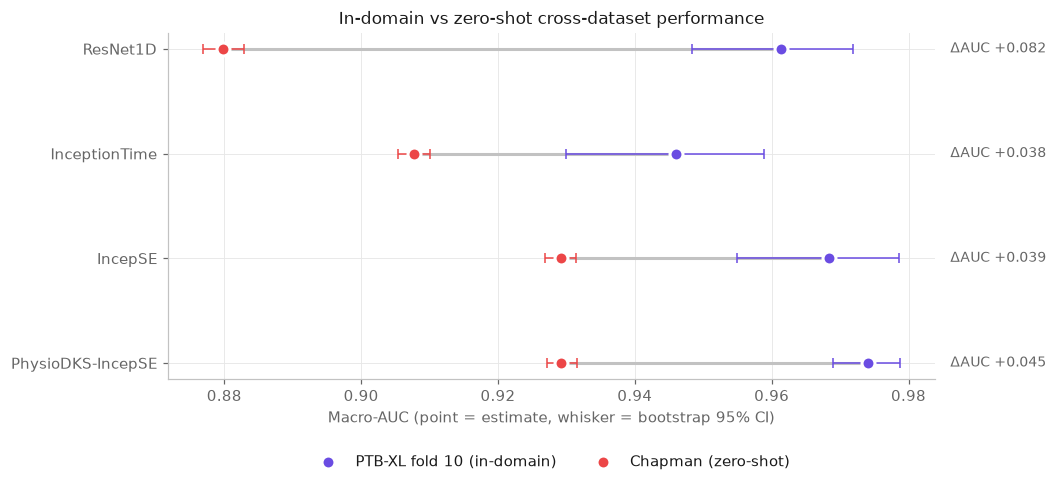
\includegraphics[width=0.8\linewidth]{figs/indomain_vs_zeroshot.png}
		\caption{Macro-AUC on PTB-XL fold 10 (in-domain) and Chapman (zero-shot), with bootstrap 95\% CI.}
	\end{figure}
\end{frame}

\begin{frame}{Results: Threshold-Based Metrics}
	\frametitle<presentation>{Threshold-Based Metrics}
	\begin{table}[h]
		\centering
		\caption{Thresholds tuned on PTB-XL fold 9 (Sens = sensitivity, Spec = specificity)}
		\renewcommand{\arraystretch}{1.2}
		\resizebox{\textwidth}{!}{
		\begin{tabular}{|l|c|c|c|c|c|c|c|}
			\hline
			\textbf{Model} & \textbf{PTB-XL F1} & \textbf{PTB-XL Sens} & \textbf{PTB-XL Spec} & \textbf{Chapman F1} & \textbf{Chapman Sens} & \textbf{Chapman Spec} & \textbf{Chapman F1 (oracle)} \\
			\hline
			ResNet1D & 0.678 & 0.700 & 0.949 & 0.439 & 0.571 & 0.921 & 0.587 \\
			\hline
			InceptionTime & 0.696 & 0.693 & 0.940 & 0.418 & 0.555 & 0.909 & 0.595 \\
			\hline
			IncepSE & 0.706 & 0.744 & 0.947 & 0.511 & 0.608 & 0.925 & 0.667 \\
			\hline
			PhysioDKS-IncepSE (proposed) & 0.710 & 0.716 & 0.950 & 0.500 & 0.572 & 0.928 & 0.669 \\
			\hline
		\end{tabular}
		}
	\end{table}
	\begin{itemize}
		\item Oracle thresholds are tuned on Chapman itself and are shown for analysis only.
		\item AUPRC and F1 depend on prevalence, so values should not be compared directly across datasets.
	\end{itemize}
\end{frame}

\begin{frame}{Results: Statistical Significance}
	\frametitle<presentation>{Statistical Significance (Paired Bootstrap, 1000 Resamples)}
	\begin{table}[h]
		\centering
		\caption{PhysioDKS-IncepSE minus each model: difference [95\% CI], p-value}
		\renewcommand{\arraystretch}{1.2}
		\resizebox{\textwidth}{!}{
		\begin{tabular}{|l|c|c|c|}
			\hline
			\textbf{Compared with} & \textbf{PTB-XL $\Delta$ Macro-AUC} & \textbf{Chapman $\Delta$ Macro-AUC} & \textbf{Gap difference (negative = better generalization)} \\
			\hline
			ResNet1D & +0.013 [+0.005, +0.022], p $<$ 0.001 & +0.050 [+0.047, +0.052], p $<$ 0.001 & $-$0.037 [$-$0.045, $-$0.027], p $<$ 0.001 \\
			\hline
			InceptionTime & +0.028 [+0.017, +0.042], p $<$ 0.001 & +0.022 [+0.020, +0.024], p $<$ 0.001 & +0.006 [$-$0.005, +0.021], p = 0.33 \\
			\hline
			IncepSE & +0.006 [$-$0.002, +0.016], p = 0.24 & +0.000 [$-$0.002, +0.002], p = 0.91 & +0.006 [$-$0.002, +0.016], p = 0.25 \\
			\hline
		\end{tabular}
		}
	\end{table}
	\begin{itemize}
		\item The proposed model is significantly better than ResNet1D and InceptionTime on both test sets.
		\item It is not significantly different from IncepSE: the gain comes mainly from the Inception + SE backbone (Chapman AUC 0.908 $\rightarrow$ 0.929), not from the Stage-1 front-end.
	\end{itemize}
\end{frame}

\begin{frame}{Results: Per-Class Performance}
	\frametitle<presentation>{Per-Class Zero-Shot AUC on Chapman}
	\begin{table}[h]
		\centering
		\renewcommand{\arraystretch}{1.2}
		\resizebox{\textwidth}{!}{
		\begin{tabular}{|l|c|c|c|c|c|c|c|c|c|}
			\hline
			\textbf{Model} & \textbf{NSR} & \textbf{AFIB} & \textbf{AFL} & \textbf{RBBB} & \textbf{LBBB} & \textbf{PAC} & \textbf{PVC} & \textbf{STach} & \textbf{SBrady} \\
			\hline
			ResNet1D & 0.842 & 0.910 & 0.677 & 0.983 & 0.898 & 0.852 & 0.954 & 0.938 & 0.864 \\
			\hline
			InceptionTime & 0.884 & 0.908 & 0.819 & 0.987 & 0.928 & 0.805 & 0.970 & 0.987 & 0.883 \\
			\hline
			IncepSE & 0.873 & 0.921 & 0.849 & 0.984 & 0.925 & 0.937 & 0.971 & 0.982 & 0.920 \\
			\hline
			PhysioDKS-IncepSE & 0.886 & 0.922 & 0.849 & 0.986 & 0.931 & 0.917 & 0.963 & 0.976 & 0.933 \\
			\hline
		\end{tabular}
		}
	\end{table}
	\begin{itemize}
		\item \textbf{AFL:} ResNet1D nearly fails (0.677); Inception-family models reach 0.82--0.85 despite only 59 training examples.
		\item \textbf{RBBB, PVC, STach:} AUC above 0.96 for Inception-family models; these classes transfer well across hospitals.
		\item \textbf{AFIB, LBBB:} similar drop for all models, which points to differences in label definitions between datasets rather than the model.
	\end{itemize}
\end{frame}

\begin{frame}{Results: Threshold Transfer}
	\frametitle<presentation>{Why F1 Drops: Threshold Transfer}
	\begin{columns}[c]
		\begin{column}{0.45\textwidth}
			\begin{itemize}
				\item Chapman AUC drops only 0.04--0.08, but macro-F1 of the proposed model drops from 0.710 to 0.500.
				\item Thresholds tuned on PTB-XL do not fit Chapman because prevalence changes (e.g. SBrady 2.9\% $\rightarrow$ 36.7\%).
				\item With Chapman-tuned (oracle) thresholds, F1 recovers to 0.669.
				\item The model's ranking ability transfers; its decision thresholds do not. Recalibration is needed for deployment.
			\end{itemize}
		\end{column}
		\begin{column}{0.53\textwidth}
			\begin{figure}[htbp]
				\centering
				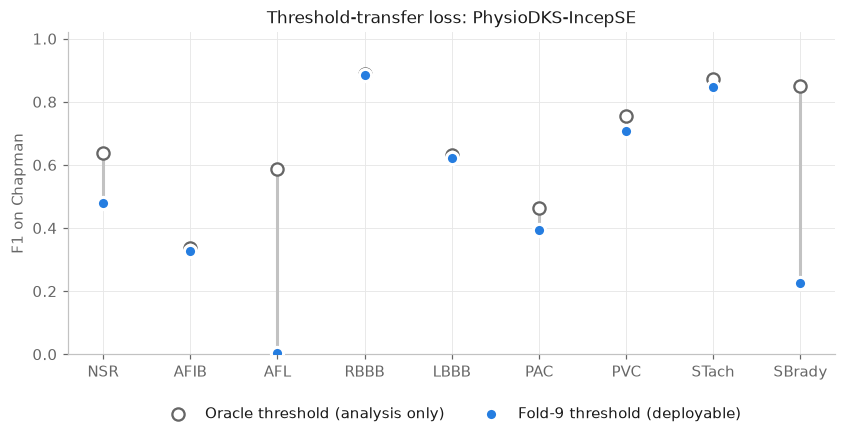
\includegraphics[width=\linewidth]{figs/threshold_transfer.png}
				\caption{Per-class Chapman F1: fold-9 threshold vs oracle threshold.}
			\end{figure}
		\end{column}
	\end{columns}
\end{frame}

% =====================================================
\section{Explainability}
% =====================================================

\begin{frame}{Explainability: Grad-CAM}
	\frametitle<presentation>{Explainability: 1D Grad-CAM Example (PVC)}
	\begin{figure}[htbp]
		\centering
		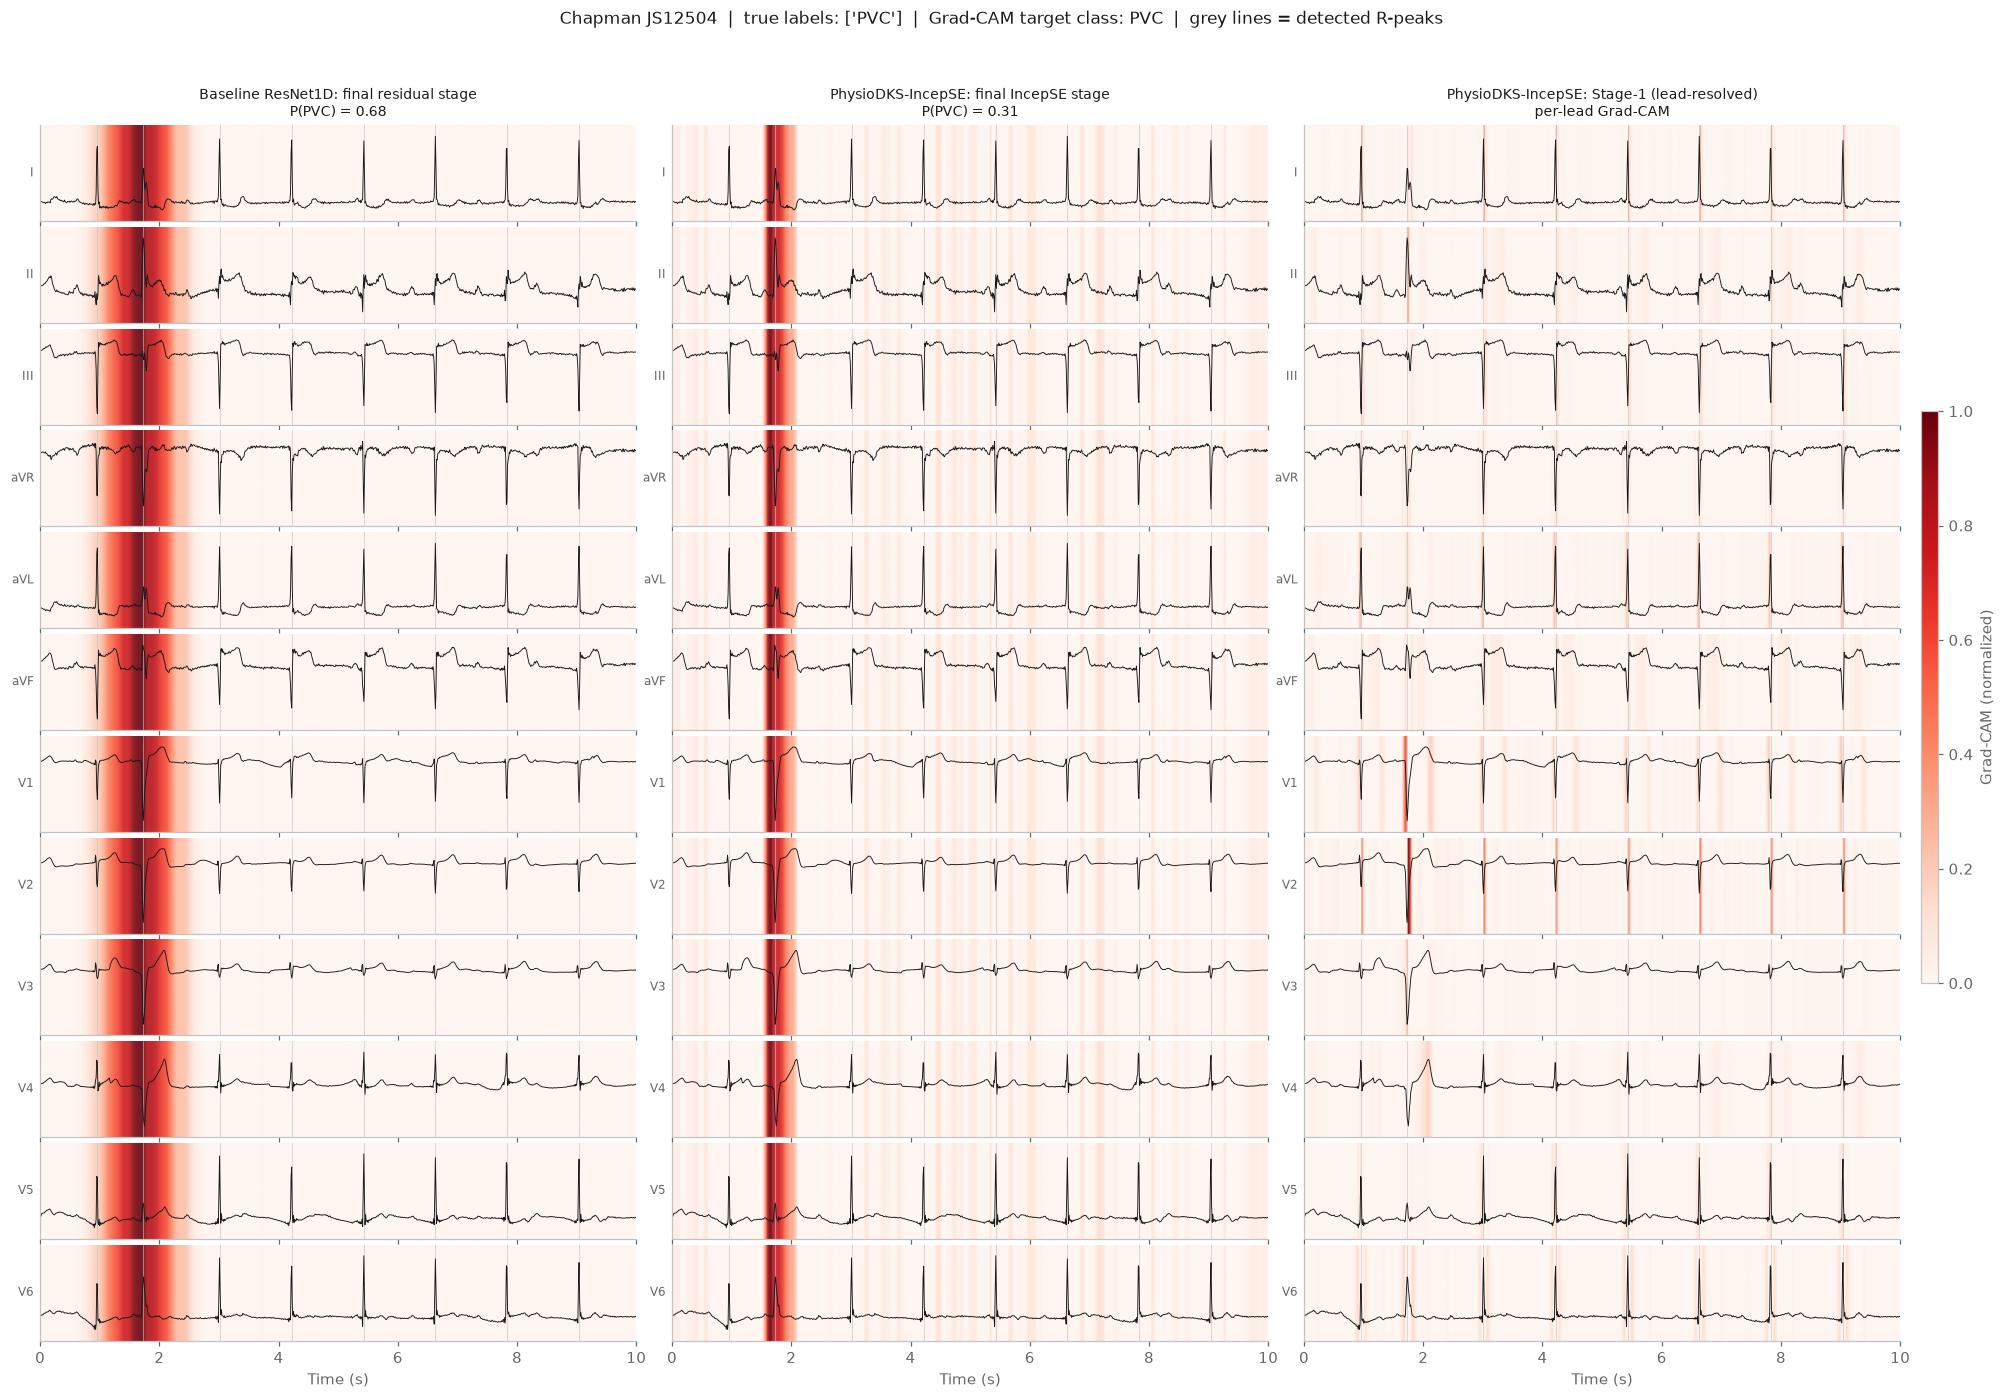
\includegraphics[width=0.48\linewidth]{figs/gradcam_pvc.png}
		\caption{Chapman JS12504 (PVC). Left: ResNet1D. Middle: proposed, final stage. Right: proposed, Stage-1 per-lead Grad-CAM \cite{selvaraju2017gradcam}.}
	\end{figure}
	\begin{itemize}
		\item The proposed model's heatmap is localized on the premature beat (about 0.3 s); ResNet1D's heatmap spreads over about 1 s. Examples were selected with a fixed random seed.
	\end{itemize}
\end{frame}

\begin{frame}{Explainability: Quantitative Saliency}
	\frametitle<presentation>{Quantitative Saliency (100 Chapman Positives per Class, Median)}
	\begin{table}[h]
		\centering
		\renewcommand{\arraystretch}{1.1}
		\resizebox{0.85\textwidth}{!}{
		\begin{tabular}{|l|c|c|c|c|c|c|c|}
			\hline
			\textbf{Class} & \textbf{QRS enr. ResNet1D} & \textbf{QRS enr. Proposed} & \textbf{QRS enr. Stage-1} & \textbf{p} & \textbf{Off-wave ResNet1D} & \textbf{Off-wave Proposed} & \textbf{p} \\
			\hline
			RBBB & 1.42 & 1.46 & 3.10 & 0.006 & 0.054 & 0.000 & $<$0.001 \\
			LBBB & 1.61 & 1.58 & 2.23 & 0.32 & 0.004 & 0.004 & 0.35 \\
			PVC & 1.06 & 1.33 & 2.71 & $<$0.001 & 0.016 & 0.011 & 0.48 \\
			PAC & 1.41 & 1.50 & 3.09 & 0.15 & 0.006 & 0.078 & $<$0.001 \\
			AFIB & 1.10 & 0.89 & 2.70 & $<$0.001 & 0.060 & 0.073 & 0.006 \\
			NSR & 1.05 & 0.32 & 2.98 & $<$0.001 & 0.157 & 0.218 & $<$0.001 \\
			STach & 1.03 & 0.59 & 2.32 & $<$0.001 & 0.000 & 0.000 & $<$0.001 \\
			SBrady & 0.00 & 0.00 & 3.54 & 0.004 & 0.802 & 0.855 & 0.37 \\
			AFL & 0.40 & 0.00 & 2.48 & n/a & 0.000 & 0.039 & n/a \\
			\hline
		\end{tabular}
		}
	\end{table}
	\begin{itemize}
		\item QRS enrichment $>$ 1 means more attention on the QRS than expected by chance. p-values: Wilcoxon test, ResNet1D vs proposed.
		\item Stage-1 is QRS-focused in every class (2.2--3.5$\times$). The proposed model focuses more on the QRS for RBBB and PVC, and on the inter-beat baseline for rhythm classes (NSR, STach, SBrady), which is clinically consistent.
	\end{itemize}
\end{frame}

\begin{frame}{Explainability: Lead Importance}
	\frametitle<presentation>{Explainability: Which Leads Matter?}
	\begin{figure}[htbp]
		\centering
		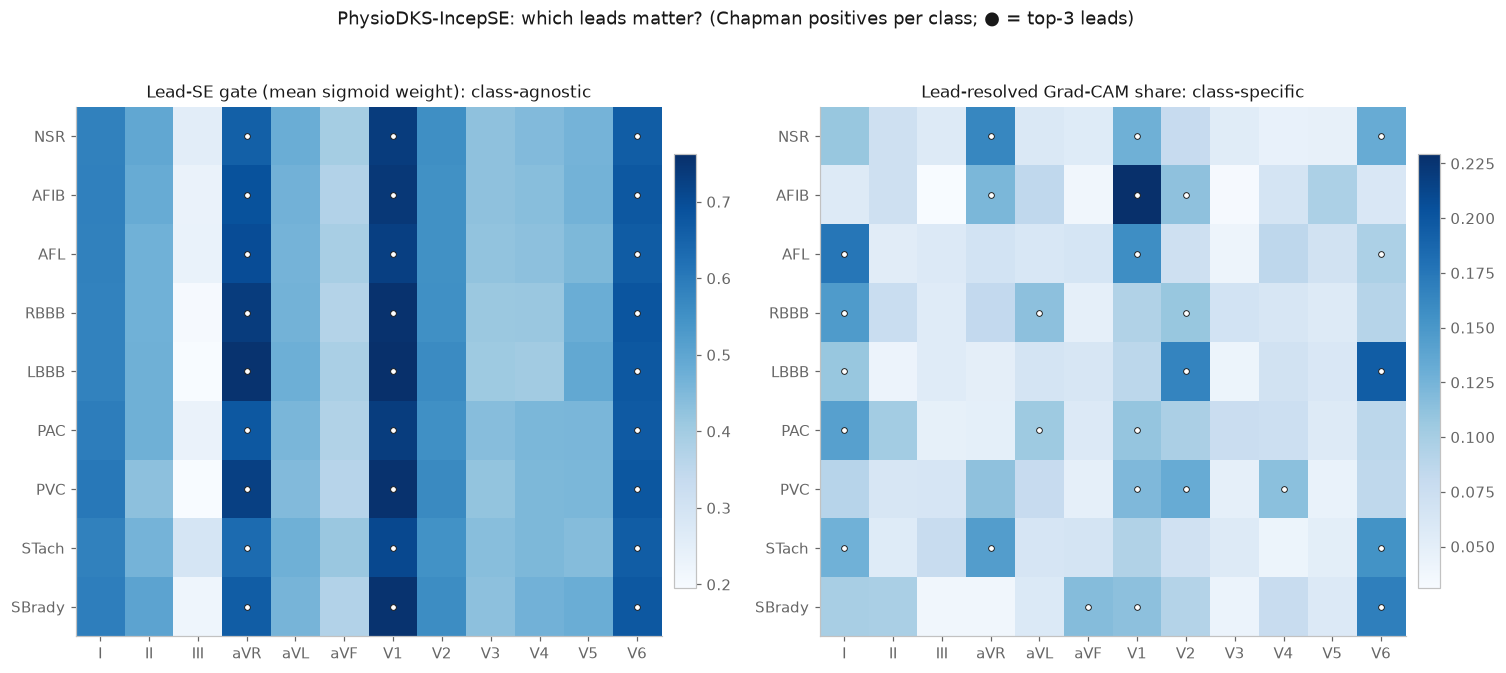
\includegraphics[width=0.62\linewidth]{figs/lead_importance.png}
		\caption{Left: Lead-SE gate weights. Right: class-wise lead-resolved Grad-CAM share.}
	\end{figure}
	\begin{itemize}
		\item Grad-CAM top leads match textbook patterns for some classes: AFIB $\rightarrow$ V1, aVR, V2; LBBB $\rightarrow$ V6, V2, I; PVC $\rightarrow$ V2, V1, V4.
		\item The Lead-SE gate is class-agnostic (V1, aVR, V6 highest for every class), so it is not a per-class explanation.
	\end{itemize}
\end{frame}

\begin{frame}{Explainability: Stage-1 Filters}
	\frametitle<presentation>{Explainability: Stage-1 Filters and Dynamic Kernel Selection}
	\begin{columns}[c]
		\begin{column}{0.45\textwidth}
			\begin{itemize}
				\item Learned filters stayed within their physiological frequency bands (spectral centroid 24.6 $\rightarrow$ 23.8 Hz, 11.6 $\rightarrow$ 11.5 Hz, 6.1 $\rightarrow$ 6.2 Hz).
				\item Leads I, V4 and V5 prefer the QRS-scale kernel (k = 5); inferior leads II and III prefer the P/T-scale kernel (k = 21).
				\item Kernel selection varies across records (branch weights about 0.32--0.37), but class-wise differences are small.
			\end{itemize}
		\end{column}
		\begin{column}{0.53\textwidth}
			\begin{figure}[htbp]
				\centering
				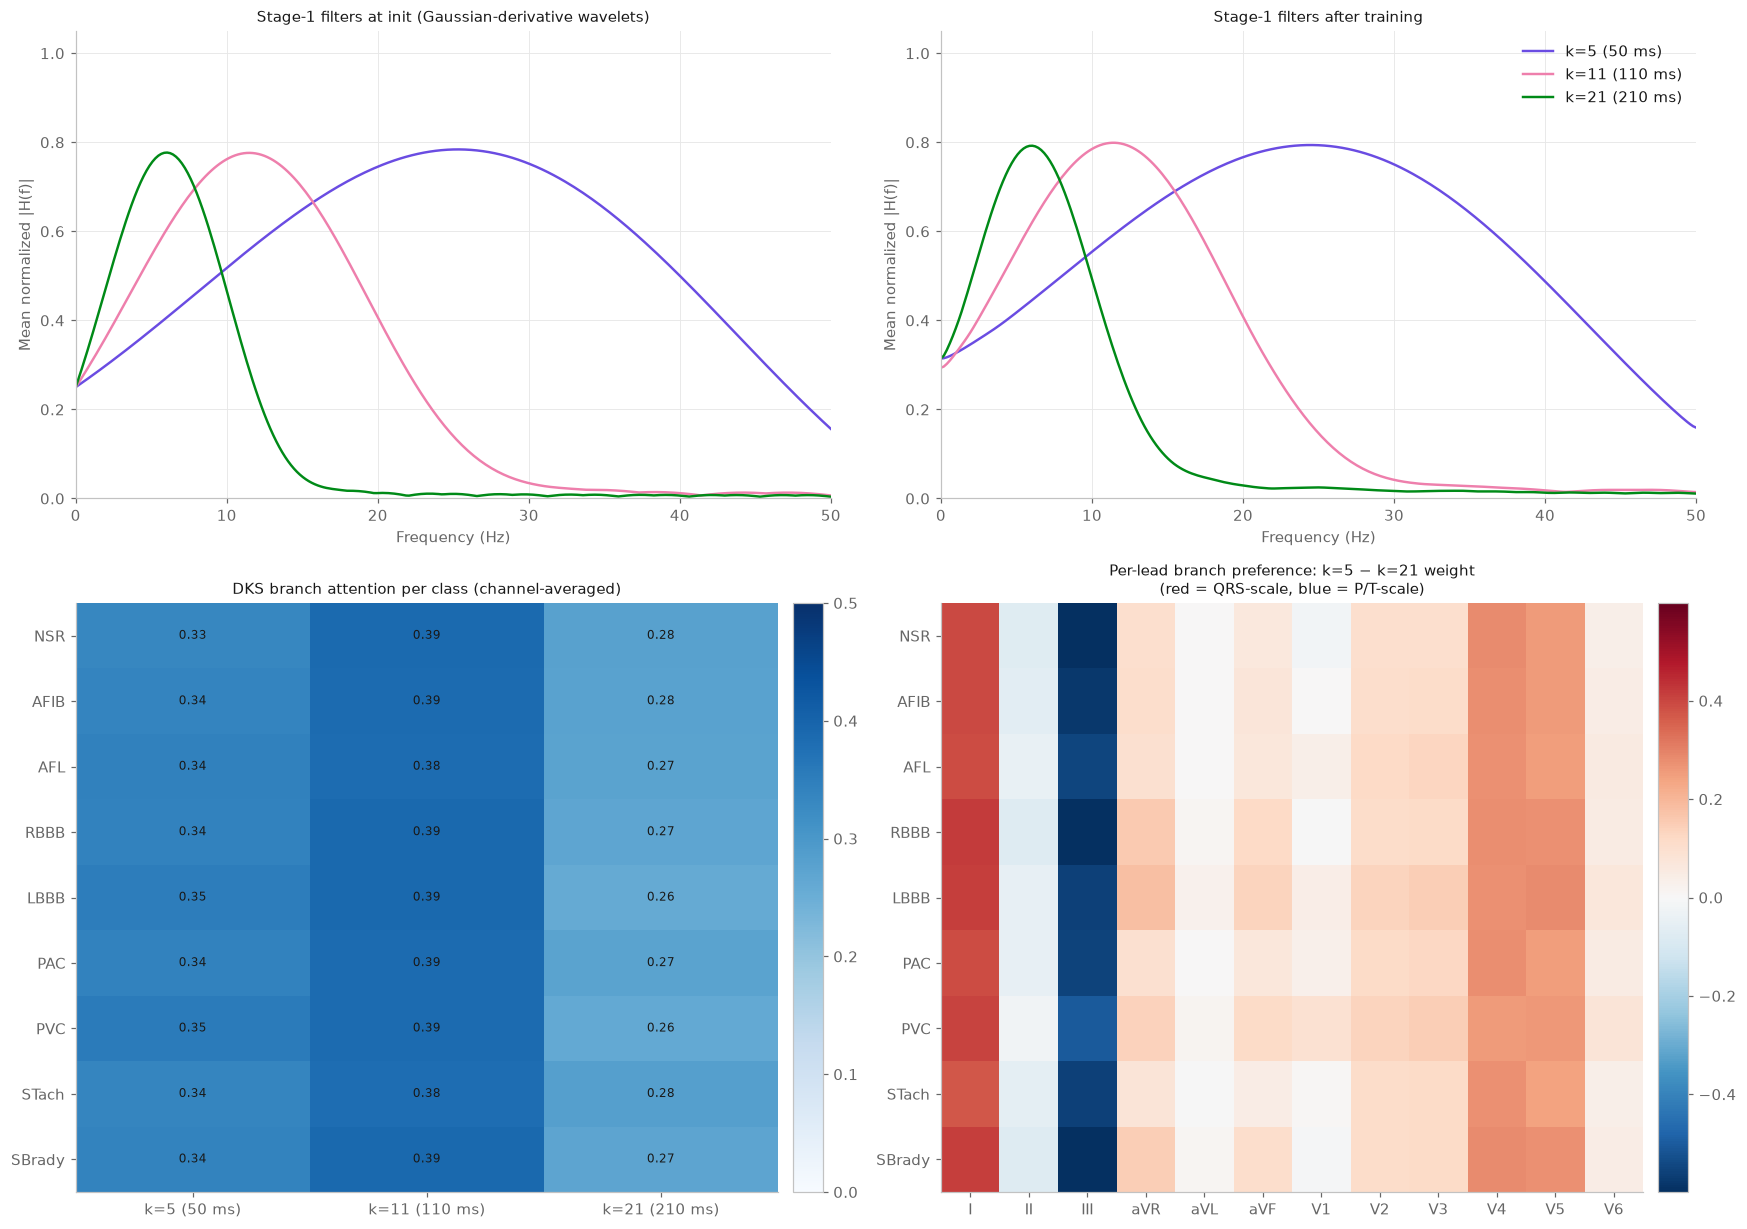
\includegraphics[width=\linewidth]{figs/dks_filters.png}
				\caption{Top: filter frequency response before and after training. Bottom: DKS attention per class and per lead.}
			\end{figure}
		\end{column}
	\end{columns}
\end{frame}

\begin{frame}{Hypothesis Summary}
	\frametitle<presentation>{Hypothesis Summary}
	\begin{table}[h]
		\centering
		\small
		\renewcommand{\arraystretch}{1.3}
		\begin{tabular}{|>{\raggedright\arraybackslash}p{0.30\textwidth}|>{\raggedright\arraybackslash}p{0.15\textwidth}|>{\raggedright\arraybackslash}p{0.45\textwidth}|}
			\hline
			\textbf{Hypothesis} & \textbf{Result} & \textbf{Evidence} \\
			\hline
			H1: ResNet1D loses the most under hospital shift & Supported & $\Delta$AUC 0.082 vs 0.038--0.045 for Inception-family models \\
			\hline
			H2: Stage-1 front-end reduces domain shift & Not supported & Gap difference vs IncepSE +0.006 [$-$0.002, +0.016], p = 0.25 \\
			\hline
			H3: Proposed model improves in-domain and cross-dataset performance & Partially supported & Better than ResNet1D and InceptionTime (p $<$ 0.001); equal to IncepSE (p = 0.24 / 0.91) \\
			\hline
			H4: Proposed model focuses on P/QRS/T waves & Partially supported & Class-dependent: stronger QRS focus for PVC and RBBB; baseline focus for rhythm classes \\
			\hline
		\end{tabular}
	\end{table}
\end{frame}

% =====================================================
\section{Conclusion}
% =====================================================

\begin{frame}{Conclusion}
	\frametitle<presentation>{Conclusion}
	\begin{itemize}
		\item \textbf{Fair zero-shot benchmark:} Four parameter-matched CNNs were trained on PTB-XL under one identical protocol and tested on 45,151 Chapman ECGs without any adaptation.
		\item \textbf{Main finding:} The Inception + SE backbone generalizes much better than a parameter-matched ResNet ($\Delta$AUC 0.039 vs 0.082). PhysioDKS-IncepSE reaches 0.974 in-domain and 0.929 zero-shot macro-AUC, but is statistically equal to IncepSE.
		\item \textbf{Threshold transfer:} Most of the external F1 loss (0.710 $\rightarrow$ 0.500) comes from thresholds that do not transfer under prevalence shift; oracle thresholds recover F1 to 0.669.
		\item \textbf{Interpretability:} The physiological front-end keeps accuracy while adding lead- and frequency-level interpretability, with class-consistent saliency patterns.
	\end{itemize}
\end{frame}

\begin{frame}{Limitations}
	\frametitle<presentation>{Limitations}
	\begin{itemize}
		\item \textbf{Single seed:} All results come from one training seed (42); confidence intervals reflect test-set sampling only, not training randomness.
		\item \textbf{Rare class:} AFL has only 59 training, 7 validation and 7 test positives in PTB-XL, so its threshold and in-domain AUC are unreliable.
		\item \textbf{Label definitions:} Chapman's LBBB code also covers fascicular blocks; the external set mixes two hospitals (Chapman-Shaoxing and Ningbo).
		\item \textbf{Residual spectral shift:} Chapman shows slightly higher power at 30--45 Hz after identical preprocessing, possibly due to different resampling pipelines.
		\item \textbf{Approximate XAI:} Grad-CAM is an approximation, and the QRS/PQRST windows are heuristic.
		\item \textbf{Benchmark comparability:} The rhythm9 task and preprocessing differ from the Strodthoff et al. benchmark \cite{strodthoff2021}, so numbers are not directly comparable with published PTB-XL results.
	\end{itemize}
\end{frame}

\begin{frame}{Future Work}
	\frametitle<presentation>{Future Work}
	\begin{itemize}
		\item Repeat all experiments with three seeds and report mean $\pm$ standard deviation.
		\item Extended ablation of Stage-1 components (DKS, InstanceNorm, Lead-SE, physiological initialization).
		\item Threshold adaptation for zero-shot deployment: temperature scaling and prevalence-adjusted thresholds.
		\item Resampling parity: process PTB-XL from 500 Hz with the same resampler as Chapman.
		\item Run the PTB-XL superdiagnostic (5-class) task for direct comparison with published literature.
	\end{itemize}
\end{frame}

% =====================================================
\section*{References}
% =====================================================

\begin{frame}[allowframebreaks]
	\frametitle<presentation>{References}
	\bibliographystyle{ieeetr}
	\bibliography{mybibfile.bib}
\end{frame}

% =====================================================
% Thank You
% =====================================================

\begin{frame}\vspace{0.6in}
	\centering
	\fontfamily{cmtt}\fontsize{60 pt}{1}\textit{\textbf{Thank You !!}}\\ \vspace{1in}
	\centering
	\fontfamily{lmr}\fontsize{20 pt}{1}
\end{frame}

\end{document}
